\documentclass{beamer}
\usepackage{lmodern}

\usetheme{Malmoe}
\usepackage{array}
\usepackage{xcolor}
\usepackage{listings} % DO NOT USE DRAFT DOCUMENT AS IT WILL NOT DISPLAY THE CODE

\usepackage{pgf,tikz}
\usetikzlibrary{arrows,automata,shapes}
%\tikzstyle{block} = [rectangle, draw, fill=blue!20, text width=5em, text centered, rounded corners, minimum height=4em]
\tikzstyle{block} = [rectangle, draw, text width=5em, text centered, rounded corners, minimum height=4em]
%\tikzstyle{pass} = [rectangle, draw, fill=blue!20, text centered, rounded corners]
\tikzstyle{pass} = [rectangle, draw, text centered, rounded corners]
\tikzstyle{txt} = [text centered]

\usetikzlibrary{positioning,calc,arrows}
\lstset{language=Oz,basicstyle=\ttfamily\small,columns=fullflexible,keepspaces=true,
escapechar=µ}

\title{A modular Oz compiler for the new 64-bit Mozart virtual machine}
\author{Rapha\"el Bauduin}
\date{26 june 2013}
\begin{document}

% \newcommand{\example}{Example}

\begin{frame}
 \titlepage
\end{frame}

\begin{frame}
 \tableofcontents
\end{frame}


\section{Introduction and Goals}

\begin{frame}
\frametitle{Origin of this work}
\begin{itemize}
  \item Mozart1 compiler was old
  \item A new virtual machine had been developed
  \item A new compiler was deemed necessary
\end{itemize}

Goals of this work
\begin{itemize}
  \item support whole Oz language
  \item generate quality code targeting the new virtual machine
  \item easy to understand and modular code
  \item obtain a compiler easy to extend
\end{itemize}
\vspace{\baselineskip}

\end{frame}

\section{The Compiler}

\begin{frame}
\frametitle{Structure of the compiler}
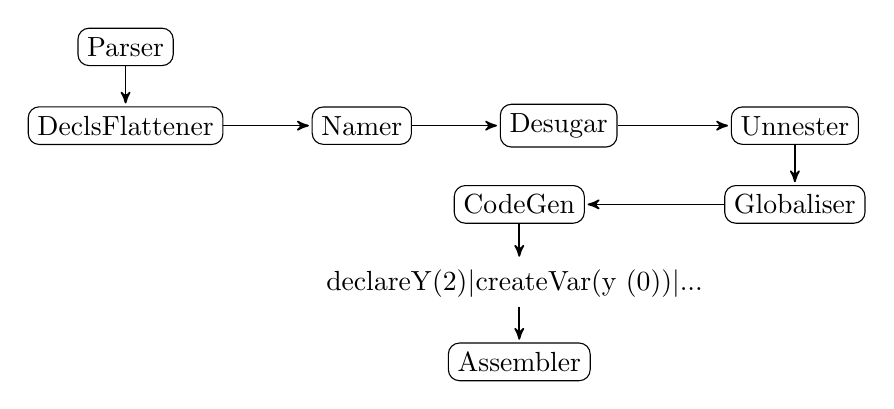
\begin{tikzpicture}[auto,every matrix/.style={ampersand replacement=\&,column sep=2cm,row sep=2cm},
                             to/.style={->,>=stealth',shorten >=1pt,semithick,font=\sffamily\footnotesize}]
  \node[pass](parser) at (0,1) {Parser};
  \node[pass](declsFlattener) at (0,0) {DeclsFlattener};
  \node[pass](namer) at (3,0) {Namer};
  \node[pass](desugar) at (5.5,0) {Desugar};
  \node[pass](unnester) at (8.5,0) {Unnester};
  \node[pass](globaliser) at (8.5,-1) {Globaliser};
  \node[pass](codegen) at (5,-1) {CodeGen};
  \node[txt](opcodes) at (5,-2) {\lstinline!declareY(2)|createVar(y(0))|...!};
  \node[pass](assembler) at (5,-3) {Assembler};

  \draw[to]  (parser.south) -- (declsFlattener.north);
  \draw[to]  (declsFlattener.east) -- (namer.west);
  \draw[to]  (namer.east) -- (desugar.west);
  \draw[to]  (desugar.east) -- (unnester.west);
  \draw[to]  (unnester.south) -- (globaliser.north);
  \draw[to]  (globaliser.west) -- (codegen.east);
  \draw[to]  (codegen.south) -- (opcodes.north);
  \draw[to]  (opcodes.south) -- (assembler.north);
\end{tikzpicture}
\end{frame}

\begin{frame}
\frametitle{Compiler passes}
\begin{description}
  \item[DeclsFlattener] Lease only declarations in declaration part of \lstinline!local..in..end!
  \item[Namer] Replace all occurrences  of a variables by 1 symbols
  \item[Desugar] E.g make features explicit, transform class and functors in function call
  \item[Unnester] Leave only basic instructions, e.g. extract complex conditions from \lstinline!if..then..else!
  \item[Globaliser] Introduce localised symbols for global variables of procedures
  \item[CodeGen] Generate opcodes
\end{description}
\end{frame}

\section{Development method}

\begin{frame}
\frametitle{Organisation}
Iterate:
\begin{itemize}
  \item Add language feature support
  \item Write tests
  \item Validate code comments
  \item Write report section
\end{itemize}

Result:
\begin{itemize}
  \item always releasable code
  \item complexity limited to currently implemented feature
  \item accurate documentation
\end{itemize}
\end{frame}

\section{Achievements}

\begin{frame}
\frametitle{Goal 1: support the whole language}
Nearly the whole language is supported: procedures, functions, classes, pattern matching, tail calls, cells, locks, functors, \ldots
\vspace{1cm}

Missing:
\begin{itemize}
  \item for loops iterating over multiple lists
  \item C-like for loops
  \item record pattern arguments having non-constant features
\end{itemize}
\end{frame}


\begin{frame}
\frametitle{Goal 2: generate quality code targeting the new VM}

\begin{itemize}
  \item Opcodes Targeting the new VM (e.g. patternMatching)
  \item But not optimised
  \item \lstinline!GenCode! is modular and documented
  \item approachable by new developer
\end{itemize}
\end{frame}


\begin{frame}
\frametitle{Goal 3: easy to understand and modular}
\begin{itemize}
  \item Code extensively documented
  \item Comments explain how things are done
  \item Report meant as a accompanying documentation
  \item Opcodes of the VM documented in report
\end{itemize}
\end{frame}


\begin{frame}
\frametitle{Goal 4: Extensible compiler}
\begin{itemize}
  \item ambitious goal: add language constructs dynamically
  \item not tested
  \item but code clean and simple, easy to adapt
\end{itemize}
\end{frame}

\section{Performance}

\begin{frame}
\frametitle{Performance measures}
\begin{itemize}
  \item Performance was not the first focus. 
  \item Still interesting to know performance
\end{itemize}

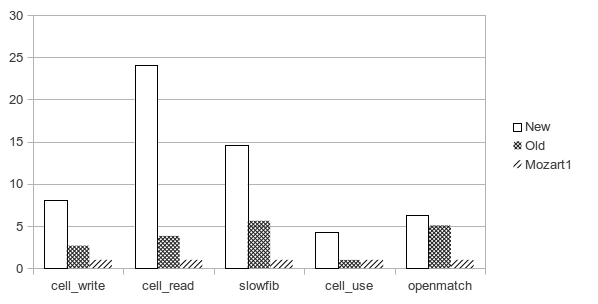
\includegraphics[scale=0.7]{../perfs/chart.png}
\end{frame}

\section{Foundation for future developments}

\begin{frame}
\frametitle{Foundation laid for future developments}
\begin{itemize}
  \item Easy to use test infrastructure
  \item Compile code, execute it, compare to expected output
  \item 439 test scripts, more than 1000 output checks
  \item Each test composed of 3 files
  \item No excuse to not write test
\end{itemize}
\end{frame}


\section{Conclusion}

\begin{frame}
\frametitle{Conclusion}
\begin{itemize}
  \item Most goals have been reached or approached
  \item Code delivered easy to understand
  \item Robust infrastructure thanks to tests
\end{itemize}
\end{frame}

\end{document}
%    \begin{block}{What is it?}
%          
%    \end{block}
